\documentclass[1p]{elsarticle_modified}
%\bibliographystyle{elsarticle-num}

%\usepackage[colorlinks]{hyperref}
%\usepackage{abbrmath_seonhwa} %\Abb, \Ascr, \Acal ,\Abf, \Afrak
\usepackage{amsfonts}
\usepackage{amssymb}
\usepackage{amsmath}
\usepackage{amsthm}
\usepackage{scalefnt}
\usepackage{amsbsy}
\usepackage{kotex}
\usepackage{caption}
\usepackage{subfig}
\usepackage{color}
\usepackage{graphicx}
\usepackage{xcolor} %% white, black, red, green, blue, cyan, magenta, yellow
\usepackage{float}
\usepackage{setspace}
\usepackage{hyperref}

\usepackage{tikz}
\usetikzlibrary{arrows}

\usepackage{multirow}
\usepackage{array} % fixed length table
\usepackage{hhline}

%%%%%%%%%%%%%%%%%%%%%
\makeatletter
\renewcommand*\env@matrix[1][\arraystretch]{%
	\edef\arraystretch{#1}%
	\hskip -\arraycolsep
	\let\@ifnextchar\new@ifnextchar
	\array{*\c@MaxMatrixCols c}}
\makeatother %https://tex.stackexchange.com/questions/14071/how-can-i-increase-the-line-spacing-in-a-matrix
%%%%%%%%%%%%%%%

\usepackage[normalem]{ulem}

\newcommand{\msout}[1]{\ifmmode\text{\sout{\ensuremath{#1}}}\else\sout{#1}\fi}
%SOURCE: \msout is \stkout macro in https://tex.stackexchange.com/questions/20609/strikeout-in-math-mode

\newcommand{\cancel}[1]{
	\ifmmode
	{\color{red}\msout{#1}}
	\else
	{\color{red}\sout{#1}}
	\fi
}

\newcommand{\add}[1]{
	{\color{blue}\uwave{#1}}
}

\newcommand{\replace}[2]{
	\ifmmode
	{\color{red}\msout{#1}}{\color{blue}\uwave{#2}}
	\else
	{\color{red}\sout{#1}}{\color{blue}\uwave{#2}}
	\fi
}

\newcommand{\Sol}{\mathcal{S}} %segment
\newcommand{\D}{D} %diagram
\newcommand{\A}{\mathcal{A}} %arc


%%%%%%%%%%%%%%%%%%%%%%%%%%%%%5 test

\def\sl{\operatorname{\textup{SL}}(2,\Cbb)}
\def\psl{\operatorname{\textup{PSL}}(2,\Cbb)}
\def\quan{\mkern 1mu \triangleright \mkern 1mu}

\theoremstyle{definition}
\newtheorem{thm}{Theorem}[section]
\newtheorem{prop}[thm]{Proposition}
\newtheorem{lem}[thm]{Lemma}
\newtheorem{ques}[thm]{Question}
\newtheorem{cor}[thm]{Corollary}
\newtheorem{defn}[thm]{Definition}
\newtheorem{exam}[thm]{Example}
\newtheorem{rmk}[thm]{Remark}
\newtheorem{alg}[thm]{Algorithm}

\newcommand{\I}{\sqrt{-1}}
\begin{document}

%\begin{frontmatter}
%
%\title{Boundary parabolic representations of knots up to 8 crossings}
%
%%% Group authors per affiliation:
%\author{Yunhi Cho} 
%\address{Department of Mathematics, University of Seoul, Seoul, Korea}
%\ead{yhcho@uos.ac.kr}
%
%
%\author{Seonhwa Kim} %\fnref{s_kim}}
%\address{Center for Geometry and Physics, Institute for Basic Science, Pohang, 37673, Korea}
%\ead{ryeona17@ibs.re.kr}
%
%\author{Hyuk Kim}
%\address{Department of Mathematical Sciences, Seoul National University, Seoul 08826, Korea}
%\ead{hyukkim@snu.ac.kr}
%
%\author{Seokbeom Yoon}
%\address{Department of Mathematical Sciences, Seoul National University, Seoul, 08826,  Korea}
%\ead{sbyoon15@snu.ac.kr}
%
%\begin{abstract}
%We find all boundary parabolic representation of knots up to 8 crossings.
%
%\end{abstract}
%\begin{keyword}
%    \MSC[2010] 57M25 
%\end{keyword}
%
%\end{frontmatter}

%\linenumbers
%\tableofcontents
%
\newcommand\colored[1]{\textcolor{white}{\rule[-0.35ex]{0.8em}{1.4ex}}\kern-0.8em\color{red} #1}%
%\newcommand\colored[1]{\textcolor{white}{ #1}\kern-2.17ex	\textcolor{white}{ #1}\kern-1.81ex	\textcolor{white}{ #1}\kern-2.15ex\color{red}#1	}

{\Large $\underline{12n_{0403}~(K12n_{0403})}$}

\setlength{\tabcolsep}{10pt}
\renewcommand{\arraystretch}{1.6}
\vspace{1cm}\begin{tabular}{m{100pt}>{\centering\arraybackslash}m{274pt}}
\multirow{5}{120pt}{
	\centering
	\includegraphics[width=112pt]{../../../GIT/diagram.site/Diagrams/png/2492_12n_0403.png}\\
\ \ \ A knot diagram\footnotemark}&
\allowdisplaybreaks
\textbf{Linearized knot diagam} \\
\cline{2-2}
 &
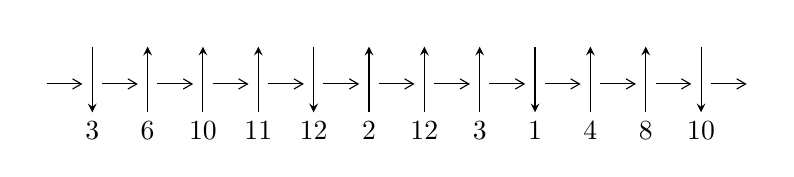
\begin{tikzpicture}[x=20pt, y=17pt]
	% nodes
	\node (C0) at (0, 0) {};
	\node (C1) at (1, 0) {};
	\node (C1U) at (1, +1) {};
	\node (C1D) at (1, -1) {3};

	\node (C2) at (2, 0) {};
	\node (C2U) at (2, +1) {};
	\node (C2D) at (2, -1) {6};

	\node (C3) at (3, 0) {};
	\node (C3U) at (3, +1) {};
	\node (C3D) at (3, -1) {10};

	\node (C4) at (4, 0) {};
	\node (C4U) at (4, +1) {};
	\node (C4D) at (4, -1) {11};

	\node (C5) at (5, 0) {};
	\node (C5U) at (5, +1) {};
	\node (C5D) at (5, -1) {12};

	\node (C6) at (6, 0) {};
	\node (C6U) at (6, +1) {};
	\node (C6D) at (6, -1) {2};

	\node (C7) at (7, 0) {};
	\node (C7U) at (7, +1) {};
	\node (C7D) at (7, -1) {12};

	\node (C8) at (8, 0) {};
	\node (C8U) at (8, +1) {};
	\node (C8D) at (8, -1) {3};

	\node (C9) at (9, 0) {};
	\node (C9U) at (9, +1) {};
	\node (C9D) at (9, -1) {1};

	\node (C10) at (10, 0) {};
	\node (C10U) at (10, +1) {};
	\node (C10D) at (10, -1) {4};

	\node (C11) at (11, 0) {};
	\node (C11U) at (11, +1) {};
	\node (C11D) at (11, -1) {8};

	\node (C12) at (12, 0) {};
	\node (C12U) at (12, +1) {};
	\node (C12D) at (12, -1) {10};
	\node (C13) at (13, 0) {};

	% arrows
	\draw[->,>={angle 60}]
	(C0) edge (C1) (C1) edge (C2) (C2) edge (C3) (C3) edge (C4) (C4) edge (C5) (C5) edge (C6) (C6) edge (C7) (C7) edge (C8) (C8) edge (C9) (C9) edge (C10) (C10) edge (C11) (C11) edge (C12) (C12) edge (C13) ;	\draw[->,>=stealth]
	(C1U) edge (C1D) (C2D) edge (C2U) (C3D) edge (C3U) (C4D) edge (C4U) (C5U) edge (C5D) (C6D) edge (C6U) (C7D) edge (C7U) (C8D) edge (C8U) (C9U) edge (C9D) (C10D) edge (C10U) (C11D) edge (C11U) (C12U) edge (C12D) ;
	\end{tikzpicture} \\
\hhline{~~} \\& 
\textbf{Solving Sequence} \\ \cline{2-2} 
 &
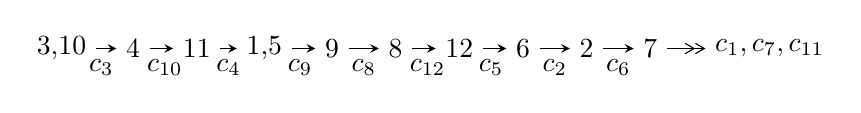
\begin{tikzpicture}[x=23pt, y=7pt]
	% node
	\node (A0) at (-1/8, 0) {3,10};
	\node (A1) at (1, 0) {4};
	\node (A2) at (2, 0) {11};
	\node (A3) at (49/16, 0) {1,5};
	\node (A4) at (33/8, 0) {9};
	\node (A5) at (41/8, 0) {8};
	\node (A6) at (49/8, 0) {12};
	\node (A7) at (57/8, 0) {6};
	\node (A8) at (65/8, 0) {2};
	\node (A9) at (73/8, 0) {7};
	\node (C1) at (1/2, -1) {$c_{3}$};
	\node (C2) at (3/2, -1) {$c_{10}$};
	\node (C3) at (5/2, -1) {$c_{4}$};
	\node (C4) at (29/8, -1) {$c_{9}$};
	\node (C5) at (37/8, -1) {$c_{8}$};
	\node (C6) at (45/8, -1) {$c_{12}$};
	\node (C7) at (53/8, -1) {$c_{5}$};
	\node (C8) at (61/8, -1) {$c_{2}$};
	\node (C9) at (69/8, -1) {$c_{6}$};
	\node (A10) at (11, 0) {$c_{1},c_{7},c_{11}$};

	% edge
	\draw[->,>=stealth]	
	(A0) edge (A1) (A1) edge (A2) (A2) edge (A3) (A3) edge (A4) (A4) edge (A5) (A5) edge (A6) (A6) edge (A7) (A7) edge (A8) (A8) edge (A9) ;
	\draw[->>,>={angle 60}]	
	(A9) edge (A10);
\end{tikzpicture} \\ 

\end{tabular} \\

\footnotetext{
The image of knot diagram is generated by the software ``\textbf{Draw programme}" developed by Andrew Bartholomew(\url{http://www.layer8.co.uk/maths/draw/index.htm\#Running-draw}), where we modified some parts for our purpose(\url{https://github.com/CATsTAILs/LinksPainter}).
}\phantom \\ \newline 
\centering \textbf{Ideals for irreducible components\footnotemark of $X_{\text{par}}$} 
 
\begin{align*}
I^u_{1}&=\langle 
- u^4-3 u^3-2 u^2+b+1,\;u^3+2 u^2+a- u-1,\;u^5+5 u^4+7 u^3+u^2-2 u-1\rangle \\
I^u_{2}&=\langle 
- u^4+u^3+2 u^2+b-2 u+1,\;u^3+a-3 u-1,\;u^5+u^4-3 u^3-3 u^2-1\rangle \\
I^u_{3}&=\langle 
- u^2 a+a u+u^2+2 b- a-3 u+1,\;u^2 a+a^2- a u-2 a+u,\;u^3-2 u^2-1\rangle \\
I^u_{4}&=\langle 
b-1,\;4 a- u-3,\;u^2- u-4\rangle \\
I^u_{5}&=\langle 
- a u+b- a+1,\;a^2- a- u+2,\;u^2- u-1\rangle \\
\\
\end{align*}
\raggedright * 5 irreducible components of $\dim_{\mathbb{C}}=0$, with total 22 representations.\\
\footnotetext{All coefficients of polynomials are rational numbers. But the coefficients are sometimes approximated in decimal forms when there is not enough margin.}
\newpage
\renewcommand{\arraystretch}{1}
\centering \section*{I. $I^u_{1}= \langle - u^4-3 u^3-2 u^2+b+1,\;u^3+2 u^2+a- u-1,\;u^5+5 u^4+7 u^3+u^2-2 u-1 \rangle$}
\flushleft \textbf{(i) Arc colorings}\\
\begin{tabular}{m{7pt} m{180pt} m{7pt} m{180pt} }
\flushright $a_{3}=$&$\begin{pmatrix}1\\0\end{pmatrix}$ \\
\flushright $a_{10}=$&$\begin{pmatrix}0\\u\end{pmatrix}$ \\
\flushright $a_{4}=$&$\begin{pmatrix}1\\- u^2\end{pmatrix}$ \\
\flushright $a_{11}=$&$\begin{pmatrix}u\\- u^3+u\end{pmatrix}$ \\
\flushright $a_{1}=$&$\begin{pmatrix}- u^3-2 u^2+u+1\\u^4+3 u^3+2 u^2-1\end{pmatrix}$ \\
\flushright $a_{5}=$&$\begin{pmatrix}- u^2+1\\u^4-2 u^2\end{pmatrix}$ \\
\flushright $a_{9}=$&$\begin{pmatrix}u^2\\- u^4-4 u^3-2 u^2+2 u+1\end{pmatrix}$ \\
\flushright $a_{8}=$&$\begin{pmatrix}u^4+4 u^3+3 u^2-2 u-1\\- u^4-4 u^3-2 u^2+2 u+1\end{pmatrix}$ \\
\flushright $a_{12}=$&$\begin{pmatrix}- u^3-2 u^2+u+1\\-2 u^4-5 u^3+2 u\end{pmatrix}$ \\
\flushright $a_{6}=$&$\begin{pmatrix}1\\- u^4-4 u^3-4 u^2+u+1\end{pmatrix}$ \\
\flushright $a_{2}=$&$\begin{pmatrix}- u^4-4 u^3-4 u^2+u+2\\u^4+3 u^3+2 u^2-1\end{pmatrix}$ \\
\flushright $a_{7}=$&$\begin{pmatrix}- u^3-2 u^2+u+1\\-2 u^4-6 u^3-3 u^2+u+1\end{pmatrix}$\\&\end{tabular}
\flushleft \textbf{(ii) Obstruction class $= -1$}\\~\\
\flushleft \textbf{(iii) Cusp Shapes $= -6 u^4-22 u^3-12 u^2+18 u+9$}\\~\\
\newpage\renewcommand{\arraystretch}{1}
\flushleft \textbf{(iv) u-Polynomials at the component}\newline \\
\begin{tabular}{m{50pt}|m{274pt}}
Crossings & \hspace{64pt}u-Polynomials at each crossing \\
\hline $$\begin{aligned}c_{1}\end{aligned}$$&$\begin{aligned}
&u^5+u^4+7 u^3+8 u^2+u-1
\end{aligned}$\\
\hline $$\begin{aligned}c_{2},c_{6},c_{7}\\c_{11}\end{aligned}$$&$\begin{aligned}
&u^5-3 u^4+5 u^3-4 u^2+3 u-1
\end{aligned}$\\
\hline $$\begin{aligned}c_{3},c_{4},c_{10}\end{aligned}$$&$\begin{aligned}
&u^5+5 u^4+7 u^3+u^2-2 u-1
\end{aligned}$\\
\hline $$\begin{aligned}c_{5},c_{9},c_{12}\end{aligned}$$&$\begin{aligned}
&u^5- u^4+12 u^3+3 u^2- u-1
\end{aligned}$\\
\hline $$\begin{aligned}c_{8}\end{aligned}$$&$\begin{aligned}
&u^5-14 u^4+51 u^3-6 u^2+4 u-13
\end{aligned}$\\
\hline
\end{tabular}\\~\\
\newpage\renewcommand{\arraystretch}{1}
\flushleft \textbf{(v) Riley Polynomials at the component}\newline \\
\begin{tabular}{m{50pt}|m{274pt}}
Crossings & \hspace{64pt}Riley Polynomials at each crossing \\
\hline $$\begin{aligned}c_{1}\end{aligned}$$&$\begin{aligned}
&y^5+13 y^4+35 y^3-48 y^2+17 y-1
\end{aligned}$\\
\hline $$\begin{aligned}c_{2},c_{6},c_{7}\\c_{11}\end{aligned}$$&$\begin{aligned}
&y^5+y^4+7 y^3+8 y^2+y-1
\end{aligned}$\\
\hline $$\begin{aligned}c_{3},c_{4},c_{10}\end{aligned}$$&$\begin{aligned}
&y^5-11 y^4+35 y^3-19 y^2+6 y-1
\end{aligned}$\\
\hline $$\begin{aligned}c_{5},c_{9},c_{12}\end{aligned}$$&$\begin{aligned}
&y^5+23 y^4+148 y^3-35 y^2+7 y-1
\end{aligned}$\\
\hline $$\begin{aligned}c_{8}\end{aligned}$$&$\begin{aligned}
&y^5-94 y^4+2441 y^3+8 y^2-140 y-169
\end{aligned}$\\
\hline
\end{tabular}\\~\\
\newpage\flushleft \textbf{(vi) Complex Volumes and Cusp Shapes}
$$\begin{array}{c|c|c}  
\text{Solutions to }I^u_{1}& \I (\text{vol} + \sqrt{-1}CS) & \text{Cusp shape}\\
 \hline 
\begin{aligned}
u &= -0.483921 + 0.312340 I \\
a &= \phantom{-}0.214528 + 0.727972 I \\
b &= -0.714557 - 0.120312 I\end{aligned}
 & -1.93405 - 1.28592 I & -1.53646 + 5.58816 I \\ \hline\begin{aligned}
u &= -0.483921 - 0.312340 I \\
a &= \phantom{-}0.214528 - 0.727972 I \\
b &= -0.714557 + 0.120312 I\end{aligned}
 & -1.93405 + 1.28592 I & -1.53646 - 5.58816 I \\ \hline\begin{aligned}
u &= \phantom{-}0.563096\phantom{ +0.000000I} \\
a &= \phantom{-}0.750397\phantom{ +0.000000I} \\
b &= \phantom{-}0.270326\phantom{ +0.000000I}\end{aligned}
 & \phantom{-}0.922645\phantom{ +0.000000I} & \phantom{-}10.8000\phantom{ +0.000000I} \\ \hline\begin{aligned}
u &= -2.29763 + 0.27249 I \\
a &= -0.08973 - 1.51845 I \\
b &= \phantom{-}0.07939 - 2.65310 I\end{aligned}
 & -13.3317 - 8.5417 I & \phantom{-}7.63666 + 3.64244 I \\ \hline\begin{aligned}
u &= -2.29763 - 0.27249 I \\
a &= -0.08973 + 1.51845 I \\
b &= \phantom{-}0.07939 + 2.65310 I\end{aligned}
 & -13.3317 + 8.5417 I & \phantom{-}7.63666 - 3.64244 I\\
 \hline 
 \end{array}$$\newpage\newpage\renewcommand{\arraystretch}{1}
\centering \section*{II. $I^u_{2}= \langle - u^4+u^3+2 u^2+b-2 u+1,\;u^3+a-3 u-1,\;u^5+u^4-3 u^3-3 u^2-1 \rangle$}
\flushleft \textbf{(i) Arc colorings}\\
\begin{tabular}{m{7pt} m{180pt} m{7pt} m{180pt} }
\flushright $a_{3}=$&$\begin{pmatrix}1\\0\end{pmatrix}$ \\
\flushright $a_{10}=$&$\begin{pmatrix}0\\u\end{pmatrix}$ \\
\flushright $a_{4}=$&$\begin{pmatrix}1\\- u^2\end{pmatrix}$ \\
\flushright $a_{11}=$&$\begin{pmatrix}u\\- u^3+u\end{pmatrix}$ \\
\flushright $a_{1}=$&$\begin{pmatrix}- u^3+3 u+1\\u^4- u^3-2 u^2+2 u-1\end{pmatrix}$ \\
\flushright $a_{5}=$&$\begin{pmatrix}- u^2+1\\u^4-2 u^2\end{pmatrix}$ \\
\flushright $a_{9}=$&$\begin{pmatrix}u^2-2\\u^4-2 u^2-1\end{pmatrix}$ \\
\flushright $a_{8}=$&$\begin{pmatrix}- u^4+3 u^2-1\\u^4-2 u^2-1\end{pmatrix}$ \\
\flushright $a_{12}=$&$\begin{pmatrix}- u^3+3 u+1\\- u^3+2 u\end{pmatrix}$ \\
\flushright $a_{6}=$&$\begin{pmatrix}-1\\u^4-2 u^2- u-1\end{pmatrix}$ \\
\flushright $a_{2}=$&$\begin{pmatrix}- u^4+2 u^2+u+2\\u^4- u^3-2 u^2+2 u-1\end{pmatrix}$ \\
\flushright $a_{7}=$&$\begin{pmatrix}u^3-3 u-1\\2 u^4-5 u^2- u-1\end{pmatrix}$\\&\end{tabular}
\flushleft \textbf{(ii) Obstruction class $= 1$}\\~\\
\flushleft \textbf{(iii) Cusp Shapes $= -2 u^4+6 u^3+4 u^2-14 u+5$}\\~\\
\newpage\renewcommand{\arraystretch}{1}
\flushleft \textbf{(iv) u-Polynomials at the component}\newline \\
\begin{tabular}{m{50pt}|m{274pt}}
Crossings & \hspace{64pt}u-Polynomials at each crossing \\
\hline $$\begin{aligned}c_{1}\end{aligned}$$&$\begin{aligned}
&u^5- u^4+3 u^3+u+1
\end{aligned}$\\
\hline $$\begin{aligned}c_{2},c_{7}\end{aligned}$$&$\begin{aligned}
&u^5- u^4+u^3+u-1
\end{aligned}$\\
\hline $$\begin{aligned}c_{3},c_{4}\end{aligned}$$&$\begin{aligned}
&u^5+u^4-3 u^3-3 u^2-1
\end{aligned}$\\
\hline $$\begin{aligned}c_{5},c_{12}\end{aligned}$$&$\begin{aligned}
&u^5- u^4- u^2+u-1
\end{aligned}$\\
\hline $$\begin{aligned}c_{6},c_{11}\end{aligned}$$&$\begin{aligned}
&u^5+u^4+u^3+u+1
\end{aligned}$\\
\hline $$\begin{aligned}c_{8}\end{aligned}$$&$\begin{aligned}
&u^5-3 u^3+6 u^2-4 u+1
\end{aligned}$\\
\hline $$\begin{aligned}c_{9}\end{aligned}$$&$\begin{aligned}
&u^5+u^4+u^2+u+1
\end{aligned}$\\
\hline $$\begin{aligned}c_{10}\end{aligned}$$&$\begin{aligned}
&u^5- u^4-3 u^3+3 u^2+1
\end{aligned}$\\
\hline
\end{tabular}\\~\\
\newpage\renewcommand{\arraystretch}{1}
\flushleft \textbf{(v) Riley Polynomials at the component}\newline \\
\begin{tabular}{m{50pt}|m{274pt}}
Crossings & \hspace{64pt}Riley Polynomials at each crossing \\
\hline $$\begin{aligned}c_{1}\end{aligned}$$&$\begin{aligned}
&y^5+5 y^4+11 y^3+8 y^2+y-1
\end{aligned}$\\
\hline $$\begin{aligned}c_{2},c_{6},c_{7}\\c_{11}\end{aligned}$$&$\begin{aligned}
&y^5+y^4+3 y^3+y-1
\end{aligned}$\\
\hline $$\begin{aligned}c_{3},c_{4},c_{10}\end{aligned}$$&$\begin{aligned}
&y^5-7 y^4+15 y^3-7 y^2-6 y-1
\end{aligned}$\\
\hline $$\begin{aligned}c_{5},c_{9},c_{12}\end{aligned}$$&$\begin{aligned}
&y^5- y^4-3 y^2- y-1
\end{aligned}$\\
\hline $$\begin{aligned}c_{8}\end{aligned}$$&$\begin{aligned}
&y^5-6 y^4+y^3-12 y^2+4 y-1
\end{aligned}$\\
\hline
\end{tabular}\\~\\
\newpage\flushleft \textbf{(vi) Complex Volumes and Cusp Shapes}
$$\begin{array}{c|c|c}  
\text{Solutions to }I^u_{2}& \I (\text{vol} + \sqrt{-1}CS) & \text{Cusp shape}\\
 \hline 
\begin{aligned}
u &= -1.48162 + 0.12936 I \\
a &= -0.266775 - 0.461665 I \\
b &= -0.54328 - 1.49449 I\end{aligned}
 & \phantom{-}6.00251 - 5.77307 I & \phantom{-}6.19041 + 5.09435 I \\ \hline\begin{aligned}
u &= -1.48162 - 0.12936 I \\
a &= -0.266775 + 0.461665 I \\
b &= -0.54328 + 1.49449 I\end{aligned}
 & \phantom{-}6.00251 + 5.77307 I & \phantom{-}6.19041 - 5.09435 I \\ \hline\begin{aligned}
u &= \phantom{-}0.099006 + 0.496292 I \\
a &= \phantom{-}1.36921 + 1.59652 I \\
b &= -0.210516 + 0.857202 I\end{aligned}
 & \phantom{-}0.38751 + 3.74061 I & \phantom{-}2.14222 - 7.10791 I \\ \hline\begin{aligned}
u &= \phantom{-}0.099006 - 0.496292 I \\
a &= \phantom{-}1.36921 - 1.59652 I \\
b &= -0.210516 - 0.857202 I\end{aligned}
 & \phantom{-}0.38751 - 3.74061 I & \phantom{-}2.14222 + 7.10791 I \\ \hline\begin{aligned}
u &= \phantom{-}1.76524\phantom{ +0.000000I} \\
a &= \phantom{-}0.795136\phantom{ +0.000000I} \\
b &= \phantom{-}0.507589\phantom{ +0.000000I}\end{aligned}
 & \phantom{-}6.95916\phantom{ +0.000000I} & \phantom{-}6.33470\phantom{ +0.000000I}\\
 \hline 
 \end{array}$$\newpage\newpage\renewcommand{\arraystretch}{1}
\centering \section*{III. $I^u_{3}= \langle - u^2 a+a u+u^2+2 b- a-3 u+1,\;u^2 a+a^2- a u-2 a+u,\;u^3-2 u^2-1 \rangle$}
\flushleft \textbf{(i) Arc colorings}\\
\begin{tabular}{m{7pt} m{180pt} m{7pt} m{180pt} }
\flushright $a_{3}=$&$\begin{pmatrix}1\\0\end{pmatrix}$ \\
\flushright $a_{10}=$&$\begin{pmatrix}0\\u\end{pmatrix}$ \\
\flushright $a_{4}=$&$\begin{pmatrix}1\\- u^2\end{pmatrix}$ \\
\flushright $a_{11}=$&$\begin{pmatrix}u\\-2 u^2+u-1\end{pmatrix}$ \\
\flushright $a_{1}=$&$\begin{pmatrix}a\\\frac{1}{2} u^2 a-\frac{1}{2} u^2+\cdots+\frac{1}{2} a-\frac{1}{2}\end{pmatrix}$ \\
\flushright $a_{5}=$&$\begin{pmatrix}- u^2+1\\2 u^2+u+2\end{pmatrix}$ \\
\flushright $a_{9}=$&$\begin{pmatrix}- u^2 a+2 a u- u^2- a\\-\frac{1}{2} u^2 a-\frac{3}{2} u^2+\cdots-\frac{1}{2} a-\frac{1}{2}\end{pmatrix}$ \\
\flushright $a_{8}=$&$\begin{pmatrix}-\frac{1}{2} u^2 a+\frac{1}{2} u^2+\cdots-\frac{1}{2} a+\frac{1}{2}\\-\frac{1}{2} u^2 a-\frac{3}{2} u^2+\cdots-\frac{1}{2} a-\frac{1}{2}\end{pmatrix}$ \\
\flushright $a_{12}=$&$\begin{pmatrix}a\\-\frac{1}{2} u^2 a-\frac{1}{2} u^2+\cdots+\frac{1}{2} a-\frac{1}{2}\end{pmatrix}$ \\
\flushright $a_{6}=$&$\begin{pmatrix}1\\-\frac{1}{2} u^2 a+\frac{1}{2} u^2+\cdots+\frac{1}{2} a-\frac{1}{2}\end{pmatrix}$ \\
\flushright $a_{2}=$&$\begin{pmatrix}-\frac{1}{2} u^2 a+\frac{1}{2} u^2+\cdots+\frac{1}{2} a+\frac{1}{2}\\\frac{1}{2} u^2 a-\frac{1}{2} u^2+\cdots+\frac{1}{2} a-\frac{1}{2}\end{pmatrix}$ \\
\flushright $a_{7}=$&$\begin{pmatrix}a\\- u^2 a+a u+u^2-2 u+1\end{pmatrix}$\\&\end{tabular}
\flushleft \textbf{(ii) Obstruction class $= -1$}\\~\\
\flushleft \textbf{(iii) Cusp Shapes $= u^2-2 u+7$}\\~\\
\newpage\renewcommand{\arraystretch}{1}
\flushleft \textbf{(iv) u-Polynomials at the component}\newline \\
\begin{tabular}{m{50pt}|m{274pt}}
Crossings & \hspace{64pt}u-Polynomials at each crossing \\
\hline $$\begin{aligned}c_{1}\end{aligned}$$&$\begin{aligned}
&u^6+8 u^4-4 u^3+8 u^2-9 u+4
\end{aligned}$\\
\hline $$\begin{aligned}c_{2},c_{6},c_{7}\\c_{11}\end{aligned}$$&$\begin{aligned}
&u^6-2 u^5+2 u^4+2 u^3-2 u^2+u+2
\end{aligned}$\\
\hline $$\begin{aligned}c_{3},c_{4},c_{10}\end{aligned}$$&$\begin{aligned}
&(u^3-2 u^2-1)^2
\end{aligned}$\\
\hline $$\begin{aligned}c_{5},c_{9},c_{12}\end{aligned}$$&$\begin{aligned}
&u^6+3 u^5+16 u^4+22 u^3+34 u^2+11 u+1
\end{aligned}$\\
\hline $$\begin{aligned}c_{8}\end{aligned}$$&$\begin{aligned}
&u^6+14 u^5+69 u^4+114 u^3+127 u^2+27 u+22
\end{aligned}$\\
\hline
\end{tabular}\\~\\
\newpage\renewcommand{\arraystretch}{1}
\flushleft \textbf{(v) Riley Polynomials at the component}\newline \\
\begin{tabular}{m{50pt}|m{274pt}}
Crossings & \hspace{64pt}Riley Polynomials at each crossing \\
\hline $$\begin{aligned}c_{1}\end{aligned}$$&$\begin{aligned}
&y^6+16 y^5+80 y^4+120 y^3+56 y^2-17 y+16
\end{aligned}$\\
\hline $$\begin{aligned}c_{2},c_{6},c_{7}\\c_{11}\end{aligned}$$&$\begin{aligned}
&y^6+8 y^4-4 y^3+8 y^2-9 y+4
\end{aligned}$\\
\hline $$\begin{aligned}c_{3},c_{4},c_{10}\end{aligned}$$&$\begin{aligned}
&(y^3-4 y^2-4 y-1)^2
\end{aligned}$\\
\hline $$\begin{aligned}c_{5},c_{9},c_{12}\end{aligned}$$&$\begin{aligned}
&y^6+23 y^5+192 y^4+540 y^3+704 y^2-53 y+1
\end{aligned}$\\
\hline $$\begin{aligned}c_{8}\end{aligned}$$&$\begin{aligned}
&y^6-58 y^5+1823 y^4+3818 y^3+13009 y^2+4859 y+484
\end{aligned}$\\
\hline
\end{tabular}\\~\\
\newpage\flushleft \textbf{(vi) Complex Volumes and Cusp Shapes}
$$\begin{array}{c|c|c}  
\text{Solutions to }I^u_{3}& \I (\text{vol} + \sqrt{-1}CS) & \text{Cusp shape}\\
 \hline 
\begin{aligned}
u &= -0.102785 + 0.665457 I \\
a &= \phantom{-}0.019191 + 0.283733 I \\
b &= -0.317796 + 1.154010 I\end{aligned}
 & \phantom{-}1.03690 + 2.56897 I & \phantom{-}6.77330 - 1.46771 I \\ \hline\begin{aligned}
u &= -0.102785 + 0.665457 I \\
a &= \phantom{-}2.31029 + 0.51852 I \\
b &= \phantom{-}0.544495 + 0.313702 I\end{aligned}
 & \phantom{-}1.03690 + 2.56897 I & \phantom{-}6.77330 - 1.46771 I \\ \hline\begin{aligned}
u &= -0.102785 - 0.665457 I \\
a &= \phantom{-}0.019191 - 0.283733 I \\
b &= -0.317796 - 1.154010 I\end{aligned}
 & \phantom{-}1.03690 - 2.56897 I & \phantom{-}6.77330 + 1.46771 I \\ \hline\begin{aligned}
u &= -0.102785 - 0.665457 I \\
a &= \phantom{-}2.31029 - 0.51852 I \\
b &= \phantom{-}0.544495 - 0.313702 I\end{aligned}
 & \phantom{-}1.03690 - 2.56897 I & \phantom{-}6.77330 + 1.46771 I \\ \hline\begin{aligned}
u &= \phantom{-}2.20557\phantom{ +0.000000I} \\
a &= -0.32948 + 1.44811 I \\
b &= -0.22670 + 2.64929 I\end{aligned}
 & -13.5883\phantom{ +0.000000I} & \phantom{-}7.45340\phantom{ +0.000000I} \\ \hline\begin{aligned}
u &= \phantom{-}2.20557\phantom{ +0.000000I} \\
a &= -0.32948 - 1.44811 I \\
b &= -0.22670 - 2.64929 I\end{aligned}
 & -13.5883\phantom{ +0.000000I} & \phantom{-}7.45340\phantom{ +0.000000I}\\
 \hline 
 \end{array}$$\newpage\newpage\renewcommand{\arraystretch}{1}
\centering \section*{IV. $I^u_{4}= \langle b-1,\;4 a- u-3,\;u^2- u-4 \rangle$}
\flushleft \textbf{(i) Arc colorings}\\
\begin{tabular}{m{7pt} m{180pt} m{7pt} m{180pt} }
\flushright $a_{3}=$&$\begin{pmatrix}1\\0\end{pmatrix}$ \\
\flushright $a_{10}=$&$\begin{pmatrix}0\\u\end{pmatrix}$ \\
\flushright $a_{4}=$&$\begin{pmatrix}1\\- u-4\end{pmatrix}$ \\
\flushright $a_{11}=$&$\begin{pmatrix}u\\-4 u-4\end{pmatrix}$ \\
\flushright $a_{1}=$&$\begin{pmatrix}\frac{1}{4} u+\frac{3}{4}\\1\end{pmatrix}$ \\
\flushright $a_{5}=$&$\begin{pmatrix}- u-3\\7 u+12\end{pmatrix}$ \\
\flushright $a_{9}=$&$\begin{pmatrix}\frac{5}{4} u+\frac{7}{4}\\2 u+1\end{pmatrix}$ \\
\flushright $a_{8}=$&$\begin{pmatrix}-\frac{3}{4} u+\frac{3}{4}\\2 u+1\end{pmatrix}$ \\
\flushright $a_{12}=$&$\begin{pmatrix}\frac{1}{4} u+\frac{3}{4}\\-2 u-3\end{pmatrix}$ \\
\flushright $a_{6}=$&$\begin{pmatrix}\frac{1}{4} u-\frac{5}{4}\\1\end{pmatrix}$ \\
\flushright $a_{2}=$&$\begin{pmatrix}\frac{1}{4} u-\frac{1}{4}\\1\end{pmatrix}$ \\
\flushright $a_{7}=$&$\begin{pmatrix}\frac{1}{2} u-\frac{3}{2}\\2\end{pmatrix}$\\&\end{tabular}
\flushleft \textbf{(ii) Obstruction class $= -1$}\\~\\
\flushleft \textbf{(iii) Cusp Shapes $= 14$}\\~\\
\newpage\renewcommand{\arraystretch}{1}
\flushleft \textbf{(iv) u-Polynomials at the component}\newline \\
\begin{tabular}{m{50pt}|m{274pt}}
Crossings & \hspace{64pt}u-Polynomials at each crossing \\
\hline $$\begin{aligned}c_{1}\end{aligned}$$&$\begin{aligned}
&(u-1)^2
\end{aligned}$\\
\hline $$\begin{aligned}c_{2},c_{6},c_{7}\\c_{11}\end{aligned}$$&$\begin{aligned}
&(u+1)^2
\end{aligned}$\\
\hline $$\begin{aligned}c_{3},c_{4},c_{10}\end{aligned}$$&$\begin{aligned}
&u^2- u-4
\end{aligned}$\\
\hline $$\begin{aligned}c_{5},c_{9},c_{12}\end{aligned}$$&$\begin{aligned}
&u^2-3 u-2
\end{aligned}$\\
\hline $$\begin{aligned}c_{8}\end{aligned}$$&$\begin{aligned}
&u^2-4 u-13
\end{aligned}$\\
\hline
\end{tabular}\\~\\
\newpage\renewcommand{\arraystretch}{1}
\flushleft \textbf{(v) Riley Polynomials at the component}\newline \\
\begin{tabular}{m{50pt}|m{274pt}}
Crossings & \hspace{64pt}Riley Polynomials at each crossing \\
\hline $$\begin{aligned}c_{1},c_{2},c_{6}\\c_{7},c_{11}\end{aligned}$$&$\begin{aligned}
&(y-1)^2
\end{aligned}$\\
\hline $$\begin{aligned}c_{3},c_{4},c_{10}\end{aligned}$$&$\begin{aligned}
&y^2-9 y+16
\end{aligned}$\\
\hline $$\begin{aligned}c_{5},c_{9},c_{12}\end{aligned}$$&$\begin{aligned}
&y^2-13 y+4
\end{aligned}$\\
\hline $$\begin{aligned}c_{8}\end{aligned}$$&$\begin{aligned}
&y^2-42 y+169
\end{aligned}$\\
\hline
\end{tabular}\\~\\
\newpage\flushleft \textbf{(vi) Complex Volumes and Cusp Shapes}
$$\begin{array}{c|c|c}  
\text{Solutions to }I^u_{4}& \I (\text{vol} + \sqrt{-1}CS) & \text{Cusp shape}\\
 \hline 
\begin{aligned}
u &= -1.56155\phantom{ +0.000000I} \\
a &= \phantom{-}0.359612\phantom{ +0.000000I} \\
b &= \phantom{-}1.00000\phantom{ +0.000000I}\end{aligned}
 & \phantom{-}8.22467\phantom{ +0.000000I} & \phantom{-}14.0000\phantom{ +0.000000I} \\ \hline\begin{aligned}
u &= \phantom{-}2.56155\phantom{ +0.000000I} \\
a &= \phantom{-}1.39039\phantom{ +0.000000I} \\
b &= \phantom{-}1.00000\phantom{ +0.000000I}\end{aligned}
 & \phantom{-}8.22467\phantom{ +0.000000I} & \phantom{-}14.0000\phantom{ +0.000000I}\\
 \hline 
 \end{array}$$\newpage\newpage\renewcommand{\arraystretch}{1}
\centering \section*{V. $I^u_{5}= \langle - a u+b- a+1,\;a^2- a- u+2,\;u^2- u-1 \rangle$}
\flushleft \textbf{(i) Arc colorings}\\
\begin{tabular}{m{7pt} m{180pt} m{7pt} m{180pt} }
\flushright $a_{3}=$&$\begin{pmatrix}1\\0\end{pmatrix}$ \\
\flushright $a_{10}=$&$\begin{pmatrix}0\\u\end{pmatrix}$ \\
\flushright $a_{4}=$&$\begin{pmatrix}1\\- u-1\end{pmatrix}$ \\
\flushright $a_{11}=$&$\begin{pmatrix}u\\- u-1\end{pmatrix}$ \\
\flushright $a_{1}=$&$\begin{pmatrix}a\\a u+a-1\end{pmatrix}$ \\
\flushright $a_{5}=$&$\begin{pmatrix}- u\\u\end{pmatrix}$ \\
\flushright $a_{9}=$&$\begin{pmatrix}a u- u+1\\a u+a\end{pmatrix}$ \\
\flushright $a_{8}=$&$\begin{pmatrix}- a- u+1\\a u+a\end{pmatrix}$ \\
\flushright $a_{12}=$&$\begin{pmatrix}a\\-1\end{pmatrix}$ \\
\flushright $a_{6}=$&$\begin{pmatrix}-1\\a u\end{pmatrix}$ \\
\flushright $a_{2}=$&$\begin{pmatrix}- a u+1\\a u+a-1\end{pmatrix}$ \\
\flushright $a_{7}=$&$\begin{pmatrix}- a\\2 a u+a- u\end{pmatrix}$\\&\end{tabular}
\flushleft \textbf{(ii) Obstruction class $= 1$}\\~\\
\flushleft \textbf{(iii) Cusp Shapes $= u+6$}\\~\\
\newpage\renewcommand{\arraystretch}{1}
\flushleft \textbf{(iv) u-Polynomials at the component}\newline \\
\begin{tabular}{m{50pt}|m{274pt}}
Crossings & \hspace{64pt}u-Polynomials at each crossing \\
\hline $$\begin{aligned}c_{1},c_{2},c_{5}\\c_{7},c_{12}\end{aligned}$$&$\begin{aligned}
&u^4- u^3+u^2- u+1
\end{aligned}$\\
\hline $$\begin{aligned}c_{3},c_{4}\end{aligned}$$&$\begin{aligned}
&(u^2- u-1)^2
\end{aligned}$\\
\hline $$\begin{aligned}c_{6},c_{9},c_{11}\end{aligned}$$&$\begin{aligned}
&u^4+u^3+u^2+u+1
\end{aligned}$\\
\hline $$\begin{aligned}c_{8}\end{aligned}$$&$\begin{aligned}
&u^4+3 u^3+4 u^2+2 u+1
\end{aligned}$\\
\hline $$\begin{aligned}c_{10}\end{aligned}$$&$\begin{aligned}
&(u^2+u-1)^2
\end{aligned}$\\
\hline
\end{tabular}\\~\\
\newpage\renewcommand{\arraystretch}{1}
\flushleft \textbf{(v) Riley Polynomials at the component}\newline \\
\begin{tabular}{m{50pt}|m{274pt}}
Crossings & \hspace{64pt}Riley Polynomials at each crossing \\
\hline $$\begin{aligned}c_{1},c_{2},c_{5}\\c_{6},c_{7},c_{9}\\c_{11},c_{12}\end{aligned}$$&$\begin{aligned}
&y^4+y^3+y^2+y+1
\end{aligned}$\\
\hline $$\begin{aligned}c_{3},c_{4},c_{10}\end{aligned}$$&$\begin{aligned}
&(y^2-3 y+1)^2
\end{aligned}$\\
\hline $$\begin{aligned}c_{8}\end{aligned}$$&$\begin{aligned}
&y^4- y^3+6 y^2+4 y+1
\end{aligned}$\\
\hline
\end{tabular}\\~\\
\newpage\flushleft \textbf{(vi) Complex Volumes and Cusp Shapes}
$$\begin{array}{c|c|c}  
\text{Solutions to }I^u_{5}& \I (\text{vol} + \sqrt{-1}CS) & \text{Cusp shape}\\
 \hline 
\begin{aligned}
u &= -0.618034\phantom{ +0.000000I} \\
a &= \phantom{-}0.50000 + 1.53884 I \\
b &= -0.809017 + 0.587785 I\end{aligned}
 & -0.657974\phantom{ +0.000000I} & \phantom{-}5.38200\phantom{ +0.000000I} \\ \hline\begin{aligned}
u &= -0.618034\phantom{ +0.000000I} \\
a &= \phantom{-}0.50000 - 1.53884 I \\
b &= -0.809017 - 0.587785 I\end{aligned}
 & -0.657974\phantom{ +0.000000I} & \phantom{-}5.38200\phantom{ +0.000000I} \\ \hline\begin{aligned}
u &= \phantom{-}1.61803\phantom{ +0.000000I} \\
a &= \phantom{-}0.500000 + 0.363271 I \\
b &= \phantom{-}0.309017 + 0.951057 I\end{aligned}
 & \phantom{-}7.23771\phantom{ +0.000000I} & \phantom{-}7.61800\phantom{ +0.000000I} \\ \hline\begin{aligned}
u &= \phantom{-}1.61803\phantom{ +0.000000I} \\
a &= \phantom{-}0.500000 - 0.363271 I \\
b &= \phantom{-}0.309017 - 0.951057 I\end{aligned}
 & \phantom{-}7.23771\phantom{ +0.000000I} & \phantom{-}7.61800\phantom{ +0.000000I}\\
 \hline 
 \end{array}$$\newpage
\newpage\renewcommand{\arraystretch}{1}
\centering \section*{ VI. u-Polynomials}
\begin{tabular}{m{50pt}|m{274pt}}
Crossings & \hspace{64pt}u-Polynomials at each crossing \\
\hline $$\begin{aligned}c_{1}\end{aligned}$$&$\begin{aligned}
&(u-1)^2(u^4- u^3+u^2- u+1)(u^5- u^4+3 u^3+u+1)\\
&\cdot(u^5+u^4+7 u^3+8 u^2+u-1)(u^6+8 u^4-4 u^3+8 u^2-9 u+4)
\end{aligned}$\\
\hline $$\begin{aligned}c_{2},c_{7}\end{aligned}$$&$\begin{aligned}
&(u+1)^2(u^4- u^3+u^2- u+1)(u^5-3 u^4+5 u^3-4 u^2+3 u-1)\\
&\cdot(u^5- u^4+u^3+u-1)(u^6-2 u^5+2 u^4+2 u^3-2 u^2+u+2)
\end{aligned}$\\
\hline $$\begin{aligned}c_{3},c_{4}\end{aligned}$$&$\begin{aligned}
&(u^2- u-4)(u^2- u-1)^2(u^3-2 u^2-1)^2(u^5+u^4-3 u^3-3 u^2-1)\\
&\cdot(u^5+5 u^4+7 u^3+u^2-2 u-1)
\end{aligned}$\\
\hline $$\begin{aligned}c_{5},c_{12}\end{aligned}$$&$\begin{aligned}
&(u^2-3 u-2)(u^4- u^3+u^2- u+1)(u^5- u^4- u^2+u-1)\\
&\cdot(u^5- u^4+12 u^3+3 u^2- u-1)(u^6+3 u^5+\cdots+11 u+1)
\end{aligned}$\\
\hline $$\begin{aligned}c_{6},c_{11}\end{aligned}$$&$\begin{aligned}
&(u+1)^2(u^4+u^3+u^2+u+1)(u^5-3 u^4+5 u^3-4 u^2+3 u-1)\\
&\cdot(u^5+u^4+u^3+u+1)(u^6-2 u^5+2 u^4+2 u^3-2 u^2+u+2)
\end{aligned}$\\
\hline $$\begin{aligned}c_{8}\end{aligned}$$&$\begin{aligned}
&(u^2-4 u-13)(u^4+3 u^3+4 u^2+2 u+1)(u^5-3 u^3+6 u^2-4 u+1)\\
&\cdot(u^5-14 u^4+51 u^3-6 u^2+4 u-13)\\
&\cdot(u^6+14 u^5+69 u^4+114 u^3+127 u^2+27 u+22)
\end{aligned}$\\
\hline $$\begin{aligned}c_{9}\end{aligned}$$&$\begin{aligned}
&(u^2-3 u-2)(u^4+u^3+u^2+u+1)(u^5- u^4+12 u^3+3 u^2- u-1)\\
&\cdot(u^5+u^4+u^2+u+1)(u^6+3 u^5+16 u^4+22 u^3+34 u^2+11 u+1)
\end{aligned}$\\
\hline $$\begin{aligned}c_{10}\end{aligned}$$&$\begin{aligned}
&(u^2- u-4)(u^2+u-1)^2(u^3-2 u^2-1)^2(u^5- u^4-3 u^3+3 u^2+1)\\
&\cdot(u^5+5 u^4+7 u^3+u^2-2 u-1)
\end{aligned}$\\
\hline
\end{tabular}\newpage\renewcommand{\arraystretch}{1}
\centering \section*{ VII. Riley Polynomials}
\begin{tabular}{m{50pt}|m{274pt}}
Crossings & \hspace{64pt}Riley Polynomials at each crossing \\
\hline $$\begin{aligned}c_{1}\end{aligned}$$&$\begin{aligned}
&(y-1)^2(y^4+y^3+y^2+y+1)(y^5+5 y^4+11 y^3+8 y^2+y-1)\\
&\cdot(y^5+13 y^4+35 y^3-48 y^2+17 y-1)\\
&\cdot(y^6+16 y^5+80 y^4+120 y^3+56 y^2-17 y+16)
\end{aligned}$\\
\hline $$\begin{aligned}c_{2},c_{6},c_{7}\\c_{11}\end{aligned}$$&$\begin{aligned}
&(y-1)^2(y^4+y^3+y^2+y+1)(y^5+y^4+3 y^3+y-1)\\
&\cdot(y^5+y^4+7 y^3+8 y^2+y-1)(y^6+8 y^4-4 y^3+8 y^2-9 y+4)
\end{aligned}$\\
\hline $$\begin{aligned}c_{3},c_{4},c_{10}\end{aligned}$$&$\begin{aligned}
&(y^2-9 y+16)(y^2-3 y+1)^2(y^3-4 y^2-4 y-1)^2\\
&\cdot(y^5-11 y^4+35 y^3-19 y^2+6 y-1)(y^5-7 y^4+15 y^3-7 y^2-6 y-1)
\end{aligned}$\\
\hline $$\begin{aligned}c_{5},c_{9},c_{12}\end{aligned}$$&$\begin{aligned}
&(y^2-13 y+4)(y^4+y^3+y^2+y+1)(y^5- y^4-3 y^2- y-1)\\
&\cdot(y^5+23 y^4+148 y^3-35 y^2+7 y-1)\\
&\cdot(y^6+23 y^5+192 y^4+540 y^3+704 y^2-53 y+1)
\end{aligned}$\\
\hline $$\begin{aligned}c_{8}\end{aligned}$$&$\begin{aligned}
&(y^2-42 y+169)(y^4- y^3+6 y^2+4 y+1)\\
&\cdot(y^5-94 y^4+2441 y^3+8 y^2-140 y-169)\\
&\cdot(y^5-6 y^4+y^3-12 y^2+4 y-1)\\
&\cdot(y^6-58 y^5+1823 y^4+3818 y^3+13009 y^2+4859 y+484)
\end{aligned}$\\
\hline
\end{tabular}
\vskip 2pc
\end{document}